\newpage
\section{Durchführung}
Der Versuch besteht aus vier verschiedenen Einzelversuchen, sodass sich die Aufteilung
in Rohrresonator-, Kugelresonator-, gekoppelter Kugelresonator- und 1-dim-Festkörper Versuchsteil gliedern lässt.

Zur Verfügung steht dabei eine PC gesteuerte Software, welche das Durchlaufen eines Schall-Frequenzspektrums 
in unterschiedlicher Schrittweite ermöglicht. Zudem lässt sich über die verwendete Software das Resonanzspektrum, welches durch das Mikrofon aufgezeichnet wird, darstellen.

Darüber hinaus kann die Frequenzmessung mit einer Schaltungseinheit
erzeugt und über ein Oszilloskop angezeigt werden.
\begin{figure}
    \center
    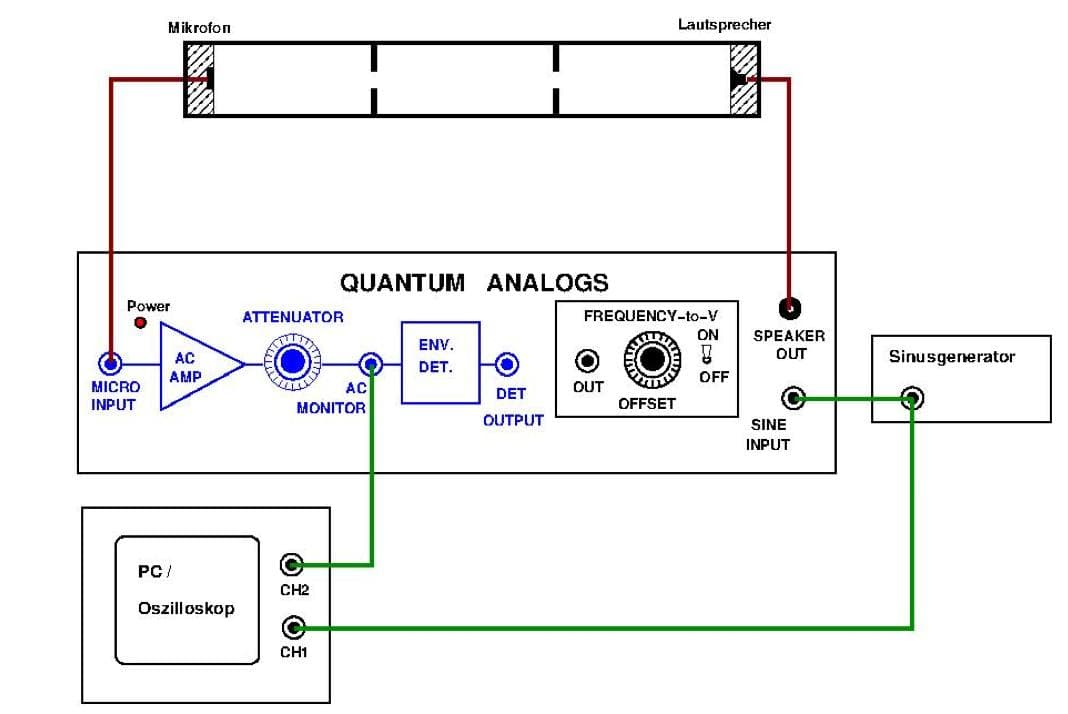
\includegraphics[width=0.7\textwidth]{bilder/anleitung.jpg}
    \caption{Schematische Darstellung der analogen Frequenzspektrum Erzeugung-/Aufnahmeschaltung.\cite{anleitung}}
\end{figure}

\subsubsection*{Auflistung der Einzelversuche}
\begin{description}
    \item Rohrresonator\\
    Vermessungen von eins bis zwölf $50\,$mm Aluminiumzylindern im Frequenzspektrum $0,10$ bis $12\,$kHz.\\
    Vermessung eines Frequenzspektrums eines einzelnen $75\,$mm Zylinders.
    \item Kugelresonator\\
    Hochauflösendes Frequenzspektrum bei einem Winkel von $180°$ (5Hz-Schritte, bei 60ms/Schritt).\\
    Druckamplitude als Funktion des Drehwinkels (Winkel in $5°$ Schritten von $0\,°$ bis $180\,°$ variieren).\\
    Vermessung der Aufspaltung beim Verwenden verschiedener Blenden.\\
    Vermessen der Winkelabhängigkeit beim Verwenden einer $9\,$mm Blende.
    \item gekoppelte Kugelresonatoren\\
    Hochauflösendes Frequenzspektrum bei verschiedenen Kopplungsstärken (Blenden).\\
    Winkelabhängigkeit bei Verwendung einer $16\,$mm Blende.\\
    \item 1-dim-Festkörper\\
    Frequenzspektrum mit verschiedener Anzahl von Zylindern und Blenden und verschiedenen Durchmessern und Längen.\\
\end{description}

\label{sec:Durchfuehrung}
